\chapter{UNIX bestandsrechten}
UNIX bestandsrechten zijn een grote bron van verwarring voor mensen die net beginnen met UNIX of op UNIX gelijkende besturingssytemen. In feite is het een simpel doch krachtig systeem. Bekijk even deze figuur:\\\\
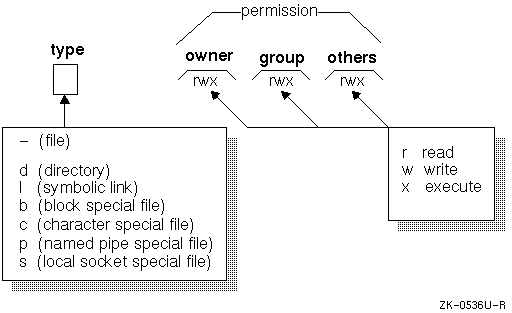
\includegraphics[scale=0.7]{src/unix_file_permissions.png}
%
Hierop zie je dat deze rechten steeds worden uitgedrukt in de vorm: 'drwxrwxrwx'. Dit kan je opdelen in een aantal verschillende stukken, namelijk: 'd rwx rwx rwx'. Hier zie je al een duidelijk onderscheid tussen de indicatie van het type bestand en de rechten die eraan worden toegewezen. Het eerste symbool (in dit geval een 'd') duidt aan wat voor type bestand je mee te maken hebt. Indien dit leeg is kan je ervan uitgaan dat je te maken hebt met een gewoon bestand. Indien je hier een 'd' tegenkomt, duidt dit erop dat het object een map is. Andere mogelijke symbolen die je waarschijnlijk niet zo vaak zal tegenkomen zijn: 'l' voor links, 'b' voor een 'block special file', 'c' voor een 'character special file', 'p' voor een 'named pipe special file' en 's' voor een 'local socket special file'. Zoals je al kon raden zijn dit veelal uitzonderingen. In de meeste gevallen zul je enkel gewone bestanden, mappen en links tegenkomen.\\\\
%
Daarnaast hebben we de 'rwx rwx rwx' structuur. Deze is in feite drie maal hetzelfde, maar geldt voor verschillende personen of groepen. De eerste iteratie duid de rechten van de eigenaar aan, de tweede iteratie is representatief voor de groep waaraan het bestand toehoort en de derde iteratie is voor publieke toegang (iedereen die niet tot \'e\'en van voorgaande groepen behoort).\\\\
De rechten zelf worden uitgedrukt in de vorm 'rwx', wat staat voor: lezen ('r'), schrijven ('w') en uitvoeren ('x'). Afhankelijk van de beschikbare waardes zal je het betreffende bestand kunnen lezen, schrijven en/of uitvoeren. Als je de rechten 'rw-' meekrijgt zal je dit bestand bijvoorbeeld zowel kunnen openen om te lezen, als wijzigingen aanbrengen. Bij de rechten 'r-x' zal je het bestand enkel kunnen lezen en uitvoeren. Dit zijn de permissies in hun simpelste vorm, maar deze zijn relatief lang om steeds op te schrijven. Daarom werd een systeem ontwikkeld waarbij deze rechten worden omgezet in cijfer. Zo krijg je voor elk van deze groepen \'e\'en cijfer, wat het een stuk compacter maakt. De waarde van deze cijfers is afhankelijk van de rechten die je erop bezit: 4 voor lezen, 2 voor schrijven en 1 voor uitvoeren. Dit zorgt ervoor dat er geen verwarring kan ontstaan over welke waarde wat betekend, aangezien alle waardes en combinaties van waardes uniek zijn. Indien je dus rechten hebt op zowel het lezen als schrijven van een bestand, worden jouw rechten opgeteld tot 6 (4 + 2). Indien je mag lezen en uitvoeren wordt dit 5 (4+1). De hoogst mogelijk rechten omvatten de mogelijkheid om zowel te lezen, schrijven en uitvoeren (rwx). Dit zorgt dan voor een totaal van 7 (4 + 2 + 1).\\\\
Deze rechten worden dan een 'mode' genoemd en worden uitgedrukt als een drie-cijferige waarde, waarbij de getallen respectievelijk de eigenaarsrechten, groepsrechten en publieke rechten omschrijven. Als je een bestand enkel toegankelijk wil maken voor jezelf, kan je dus een waarde opgeven van '700', wat ervoor zorgt dat je zelf alles kan doen met je bestand maar het niet toegankelijk is voor andere mensen. Een waarde van '644' zorgt er dan weer voor dat je zelf een bestand kan uitlezen en wijzigen, maar al de rest enkel het bestand kan uitlezen. 
